\section{Multi-Modal Dataset and Preprocessing Pipeline}
\label{sec:dataset}

To benchmark \textbf{RelieF-CR} under realistic tropical operational conditions, we constructed a heterogeneous multi-modal dataset comprising four co-registered sensor modalities across diverse agro-ecological zones and varied topography in India.

\begin{figure*}[!t]
\centering
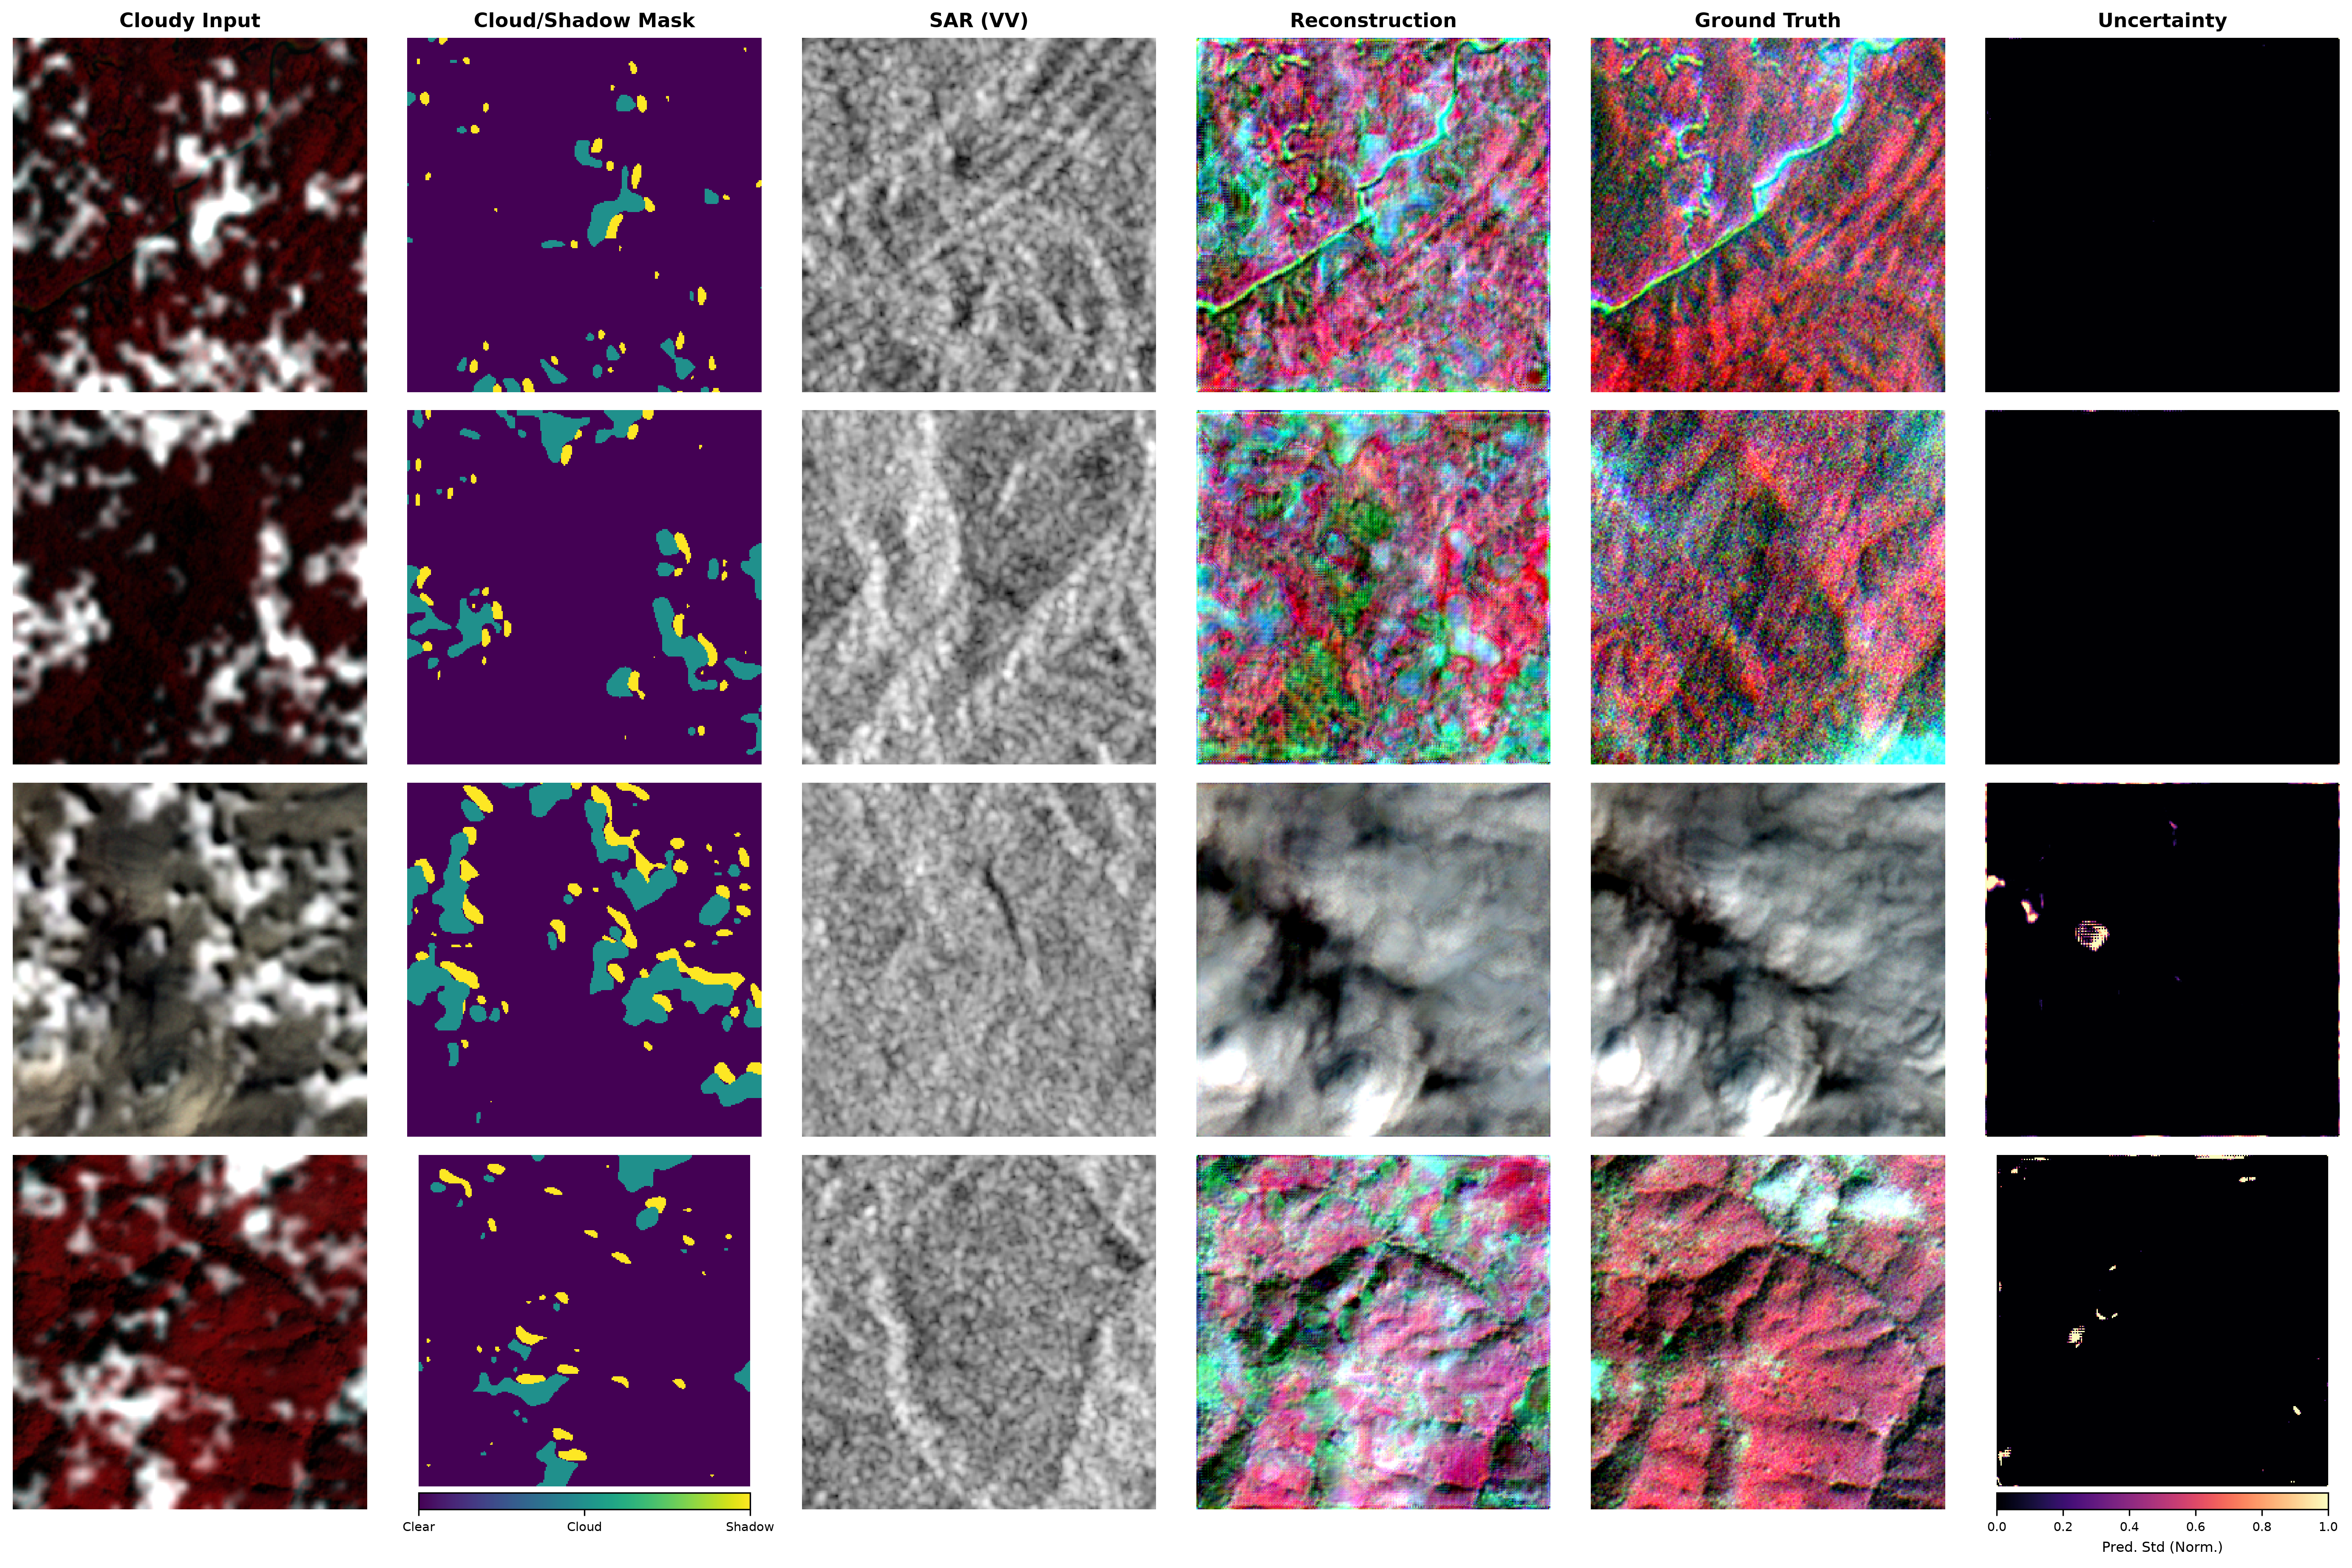
\includegraphics[width=0.98\textwidth]{figures/comparison_grid_enhanced.png}
\caption{\textbf{Qualitative Multi-Modal Cloud Removal Showcase Across Diverse High-Resolution Test Scenes.} Columns (a) to (f) depict: (a) Input cloudy LISS-IV optical composite (NIR-Red-Green false-color infrared with 2\%--98\% percentile contrast stretch), (b) Cloud/shadow 3-class segmentation mask (Clear, Cloud, Shadow), (c) Co-registered Sentinel-1 C-band SAR VV backscatter, (d) RelieF-CR reconstructed clear-sky optical reflectance $\hat{\mathbf{y}}$, (e) Ground truth 100\% clear-sky optical reference $\mathbf{y}$, and (f) Model-predicted aleatoric uncertainty standard deviation map ($\sigma = \exp(0.5 \cdot \mathbf{s})$). Across varying cloud patterns, the model eliminates dense cloud and shadow occlusions and faithfully recovers fine parcel boundaries, irrigation networks, and natural forest canopies with high structural fidelity.}
\label{fig:qualitative_grid}
\end{figure*}

\subsection{Multi-Sensor Data Ingestion \& Physical Radiometric Calibration}
The dataset integrates four complementary sensor streams:

\subsubsection{High-Resolution ISRO LISS-IV Multispectral Optical Data}
Optical scenes were acquired by the Linear Imaging Self-Scanning Sensor (LISS-IV) onboard ISRO's Resourcesat-2/2A satellites at $5.0\,\text{m}$ spatial resolution. LISS-IV provides three spectral bands: Band 2 (Green: $0.52 - 0.59\,\mu\text{m}$), Band 3 (Red: $0.62 - 0.68\,\mu\text{m}$), and Band 4 (Near-Infrared: $0.77 - 0.86\,\mu\text{m}$). Raw digital numbers ($\text{DN}$) were converted to physical Top-of-Atmosphere (TOA) spectral reflectance ($\rho_{\lambda}$) using band-specific calibration gains $G_{\lambda}$, biases $B_{\lambda}$, solar zenith angle $\theta_s$, and Earth-Sun distance correction $d$:
\begin{align}
    L_{\lambda} &= \text{DN}_{\lambda} \cdot G_{\lambda} + B_{\lambda} \\
    \rho_{\lambda} &= \frac{\pi \cdot L_{\lambda} \cdot d^2}{\text{ESUN}_{\lambda} \cdot \cos\theta_s}
\end{align}
TOA reflectance values were normalized to the dynamic range $[-1, +1]$ for network ingestion.

\subsubsection{Sentinel-1 C-Band Dual-Polarization SAR}
Same-day or nearest-pass Sentinel-1 Ground Range Detected (GRD) products were acquired in Interferometric Wide (IW) swath mode. The dual-polarization amplitude channels (VV and VH) were geocoded and resampled to the $5.0\,\text{m}$ LISS-IV master grid via bilinear Warped Virtual Raster Tables (WarpedVRT). Amplitude digital numbers were normalized via log-compression and linear mapping to $[-1, +1]$:
\begin{align}
    \tilde{x}_p &= \log_{10}\left( \text{clip}(\text{DN}_p, \text{DN}_{\min}^{(p)}, \text{DN}_{\max}^{(p)}) \right) \\
    x_{\text{sar}}^{(p)} &= 2.0 \cdot \frac{\tilde{x}_p - \log_{10}(\text{DN}_{\min}^{(p)})}{\log_{10}(\text{DN}_{\max}^{(p)}) - \log_{10}(\text{DN}_{\min}^{(p)})} - 1.0
\end{align}
where $p \in \{\text{VV}, \text{VH}\}$ with empirical clipping bounds $[\text{DN}_{\min}^{(\text{VV})}, \text{DN}_{\max}^{(\text{VV})}] = [5, 800]$ and $[\text{DN}_{\min}^{(\text{VH})}, \text{DN}_{\max}^{(\text{VH})}] = [2, 400]$, preserving microwave texture without boundary fill artifacts.

\subsubsection{CartoDEM High-Precision Topographic Surface Descriptors}
To provide explicit physical relief constraints, we incorporated the Cartosat-1 Digital Elevation Model (CartoDEM) at $10.0\,\text{m}$ resolution, resampled to the $5.0\,\text{m}$ master grid. In addition to min-max normalized elevation $z_{\text{norm}} \in [0, 1]$, we applied Horn's algorithm \cite{horn1981hill} over $3\times 3$ local windows to compute physical surface slope $S$ and topographic aspect $\Phi$:
\begin{align}
    p &= \frac{\partial z}{\partial x}, \quad q = \frac{\partial z}{\partial y} \\
    S &= \arctan\sqrt{p^2 + q^2}, \quad \Phi = \text{atan2}(-q, p)
\end{align}
Slope values are scaled to $S_{\text{norm}} \in [0, 1]$. To avoid angular discontinuity artifacts at $\Phi = 0 \equiv 2\pi$, aspect is decomposed into continuous sine and cosine projections ($\sin\Phi, \cos\Phi \in [-1, 1]$), producing a 4-channel topographic descriptor $\mathbf{X}_{\text{dem}} = [z_{\text{norm}}, S_{\text{norm}}, \sin\Phi, \cos\Phi] \in ([0, 1]^2 \times [-1, 1]^2)^{H \times W}$.

\subsubsection{Sentinel-2 Dry-Season Clear-Sky Temporal Prior}
For each scene, a cloud-free Level-2A surface reflectance product from the preceding dry season (December--February) was retrieved from the Sentinel-2 archive. Bands B03 (Green), B04 (Red), and B08 (NIR) at $10.0\,\text{m}$ resolution were projected and super-resolved to the $5.0\,\text{m}$ LISS-IV grid via bilinear WarpedVRT, with Processing Baseline $\ge 04.00$ radiometric offset correction applied, forming the baseline temporal reference $\mathbf{X}_{\text{temp}} \in [-1, 1]^{3 \times H \times W}$.

\subsection{Organic Atmospheric Cloud and Shadow Synthesis}
To construct full-reference ground truth paired data for Regime A evaluation, realistic synthetic cloud and shadow fields were simulated over clear-sky LISS-IV base tiles. We generated multi-octave fractal Perlin noise fields combining four spatial frequencies ($2, 4, 8, 16$ octaves) to model natural cloud morphology with soft, diffuse boundaries. A solar ray-tracing model projected directional cloud shadows shifted along the physical solar azimuth angle $\theta_{\text{azim}}$, modulating optical ground illumination:
\begin{equation}
    \mathbf{X}_{\text{cloudy}} = (1 - \mathbf{M}) \odot \mathbf{X}_{\text{clean}} (1 - \beta \mathbf{S}) + \mathbf{M} \odot \mathbf{C}_{\text{cloud}}
\end{equation}
where $\mathbf{M} \in [0, 1]$ is the continuous cloud opacity mask, $\mathbf{S} \in [0, 1]$ is the shadow attenuation field, $\beta \sim \mathcal{U}(0.4, 0.7)$ represents the stochastic shadow attenuation depth, and $\mathbf{C}_{\text{cloud}}$ is the atmospheric scattering color vector. The primary evaluation mask $\mathbf{M} \in [0, 1]$ represents continuous cloud opacity. While directional cloud shadows ($\mathbf{S}$) attenuate surface radiance during synthetic image formation, quantitative evaluation in this benchmark is focused on the cloud-occluded footprint, and shadow-only regions are not separately evaluated.

\subsection{Dataset Partitioning and Accounting}
The dataset contains a total of \textbf{15,480 multi-modal patches} ($256\times 256$ pixels at $5.0\,\text{m}$ GSD). Spatial non-overlapping quadrant splitting was enforced across scenes to evaluate intra-scene generalization across diverse agricultural ecotopes and complex topography:
\begin{itemize}
    \item \textbf{Training Set:} 11,950 patches ($77.2\%$)
    \item \textbf{Validation Set:} 1,919 patches ($12.4\%$)
    \item \textbf{Test Set:} 1,611 held-out patches ($10.4\%$)
\end{itemize}
All six sensor modalities (cloudy optical, clean optical, SAR, temporal reference, DEM, and cloud mask) share identical patch identifiers across all partitions. Scene-independent cross-validation across distinct satellite orbits remains an objective for future continental-scale expansions.
